\chapter{Methodology and System Design}
\label{ch:methodology}

This chapter establishes everything the evaluation chapter consumes: the datasets and their roles (Section~\ref{sec:datasets}), the evaluation protocol and its justifications (Section~\ref{sec:eval_protocol}), the data-leakage audit (Section~\ref{sec:svanstrom_audit}), the training recipes (Section~\ref{sec:training_recipes}), the human-in-the-loop data engine (Section~\ref{sec:hitl_method}), the reproducibility layer (Section~\ref{sec:reproducibility}), the Model MRI instrument (Section~\ref{sec:model_mri}), and, building on these, the system architecture and the design of each component (Section~\ref{ch:architecture}). Results live in Chapter~\ref{ch:hitl}; where a design decision below was driven by a measurement, the key number is quoted inline with a forward reference to its table: the IoP matching rule by the loose-box annotation audit (Section~\ref{sec:metrics}), the \texttt{imgsz=1280} requirement by the Svanstr\"om resolution sweep (Section~\ref{sec:resolution_arch}), and the alert-gate placement of the confuser filter by the segment-level gain on real video (Section~\ref{sec:alert_gate}).

\section{Datasets and Their Roles}
\label{sec:datasets}

The evaluation uses eight labelled corpora and a 19-clip YouTube real-video set, drawn from public benchmarks, Roboflow / Kaggle sources, and the deployment partner's CCTV stream. Each corpus plays one declared role: a training surface, an in-distribution test surface, or an out-of-distribution (OOD) stress surface. Full provenance is in Appendix~\ref{app:datasets}.

\begin{table}[htbp]
    \centering
    \caption{Evaluation surfaces and their roles. ``Role'' distinguishes training surfaces, in-distribution evaluation surfaces, and OOD stress surfaces; no OOD surface contributes any training data. Benchmark and stress surfaces are evaluation-only and carry no split.}
    \label{tab:datasets}
    \footnotesize
    \begin{tabular}{lrllp{4.0cm}}
        \toprule
        Tag & Frames & Train / val / test & Modality & Role \\
        \midrule
        \texttt{rgb\_dataset} (composite RGB corpus) & 172,022 & 137{,}506 / 17{,}307 / 17{,}209 & RGB & RGB-detector train + in-distribution test \\
        \texttt{ir\_dset\_final} & 129,130 & 107{,}809 / 11{,}709 / 9{,}612 & IR & IR-detector train + in-distribution test \\
        \texttt{rgb\_confusers\_merged} & 27,024 & 21{,}784 / 2{,}607 / 2{,}633 & RGB & Confuser hard-negative training source + OOD confuser test (test split; see Section~\ref{sec:ds_confusers} for the per-model OOD status) \\
        \texttt{IR\_confusers} & 5,938 & --- (eval-only) & IR & OOD thermal-confuser test (airplane 4{,}281 / bird 1{,}200 / helicopter 457; evaluated split 5{,}237); no training contribution \\
        \texttt{svanstrom} (paired) & 28,710 & --- (eval-only) & RGB+IR & Discriminating benchmark (small drones; labelled confusers) \\
        \texttt{antiuav} (RGBT) & 85,374 & --- (eval-only) & RGB+IR & Saturated benchmark / no-harm control \\
        \texttt{selcom\_cctv} & 2,076 & 80 / 20 split (val 311 evaluated) & RGB & Deployment-partner CCTV (fine-tune surface + held-out val) \\
        YouTube real-video diagnostic & 2,609 & --- (eval-only) & RGB & Real-world clips: drone-positive (9) + confuser-only (10); consecutive frames carry the temporal evaluation \\
        \bottomrule
    \end{tabular}
    \normalsize
\end{table}
% [source: G:/drone/dataset/dataset/dataset.yaml (137,506/17,307/17,209); G:/drone/IR_dset_final/dataset.yaml (107,809/11,709/9,612); rgb_confusers_merged/dataset_documentation.md; selcom manifest]

\begin{figure}[htbp]
    \centering
    
\includegraphics[width=\textwidth]{fig_datasets_pie}
    \caption{Global composition of the data used in this thesis. (a) Training corpora (327{,}619 frames; counts from Tables~\ref{tab:ds_rgb_components}--\ref{tab:ds_ir_components} and Appendix~\ref{app:datasets}). (b) Canonical evaluation surfaces by source size (151{,}695 frames); the Tier-1 protocol evaluates an even-spread subset of at most 4{,}000 frames per surface (Section~\ref{sec:canonical_configs}).}
    \label{fig:datasets_pie}
\end{figure}
% [source: thesis_eval/gen_dataset_figures.py (counts from the dataset tables; eval n_source from tier1_results.json)]

\begin{figure}[htbp]
    \centering
    
\includegraphics[width=0.92\textwidth]{fig_dataset_montage}
    \caption{Ground-truth drone crops across datasets and modalities (red box $=$ GT; window $\approx 4\times$ the box). Svanstr\"om drones are $19$--$29$~px small silhouettes against open sky (the regime that makes birds and distant aircraft hard to separate and that drives the cascade), while Anti-UAV drones are an order of magnitude larger; the thermal (IR) view renders the same target as a bright blob rather than a dark silhouette (Section~\ref{sec:design_rationale}).}
    \label{fig:dataset_montage}
\end{figure}

\subsection{Composite RGB Training Corpus (\texttt{rgb\_dataset})}
\label{sec:ds_rgb_corpus}

The RGB detector's training and in-distribution test corpus is a composite of nine public sources totalling 172{,}022 frames split 80/10/10 (137{,}506 train, 17{,}307 val, 17{,}209 test), sequence-disjoint. Of these, 134{,}339 (78.1\%) carry at least one drone box and 37{,}683 (21.9\%) are background negatives; the corpus contains 146{,}540 drone-class boxes. Per-source breakdown:
% [source: dataset=rgb_dataset; file=rgb_dataset/dataset.yaml (filename-prefix manifest)]

\begin{table}[htbp]
    \centering
    \caption{Per-source composition of the composite RGB training corpus. Negatives include VIRAT surveillance, UA-DETRAC traffic, and BDD100K driving frames as background contrast.}
    \label{tab:ds_rgb_components}
    \begin{tabular}{lrp{7.2cm}}
        \toprule
        Source prefix & Count & Description \\
        \midrule
        \texttt{anti}                 & 59{,}413 & Anti-UAV benchmark (CVPR 2020 / 2021)~\cite{jiang2021antiuav} RGB frames \\
        \texttt{wosdetc}              & 53{,}259 & WosDetC drone corpus \\
        \texttt{anti-muav-roboflow}   & 14{,}652 & Anti-mUAV Roboflow community variant \\
        \texttt{AirBird}              & 10{,}000 & AirBird drone-vs-bird dataset (supplies bird negatives at training time) \\
        \texttt{FBD-SV}               &  9{,}754 & Fine-grained Bird Detection (Sky View) \\
        \texttt{mav}                  &  9{,}744 & MAV (Micro Aerial Vehicle) frames \\
        \texttt{dut}                  &  5{,}200 & DUT aerial imagery \\
        \texttt{VIRAT}                &  3{,}334 & VIRAT surveillance benchmark (background negatives) \\
        \texttt{UA-DETRAC}            &  3{,}333 & UA-DETRAC traffic benchmark (background negatives) \\
        \texttt{BDD100K}              &  3{,}333 & BDD100K driving dataset (background negatives) \\
        \midrule
        \textbf{Total}                & \textbf{172{,}022} & 80/10/10 split; \texttt{drone} is the only positive class \\
        \bottomrule
    \end{tabular}
\end{table}

The bird hard negatives that make the baseline meaningful rather than a strawman come from three channels: the dedicated \texttt{AirBird} subset, the bird-focused \texttt{FBD-SV} video frames, and the bird instances of \texttt{WosDetC}, all treated as background during training. \emph{No Svanstr\"om frames of any class appear in this corpus}, nor in any other RGB training corpus of this thesis (the fine-tune chain adds SelCom and non-Svanstr\"om confuser material only, Section~\ref{sec:selcom_finetune}); Svanstr\"om is therefore fully out-of-distribution for every RGB detector variant, drones and confusers alike (Section~\ref{sec:svanstrom_audit}).
% [source: G:/drone/dataset/dataset/dataset.yaml (source prefixes: no svan); training/dataset_preparation/build_selcom_confuser_ft4.py ("No Svanström data in training"); D:/Downloads/Drone_detection_report.pdf §2.1 (WosDetC birds as background; FBD-SV as FP suppression)]

\subsection{Confuser Hard-Negative Corpus (\texttt{rgb\_confusers\_merged})}
\label{sec:ds_confusers}

The hard-negative training source for the \texttt{hardneg\_v3more} and \texttt{retrained\_v2} variants, and the OOD RGB-confuser test split. 27{,}024 images, all with empty YOLO labels, from seven sources split 80/10/10 (21{,}784 train, 2{,}607 val, 2{,}633 test). Sources without existing splits were divided by video / sequence ID to prevent temporal leakage (Svanstr\"om: 165 sequences; raihanrsd Kaggle: 58 folders; Helicopter Kaggle: hash-based pseudo-groups).

\begin{table}[htbp]
    \centering
    \caption{Per-source composition of the RGB confuser hard-negative corpus. The test split (right column) is the \emph{OOD RGB-confuser} evaluation surface used in Chapter~\ref{ch:hitl}.}
    \label{tab:ds_confusers}
    \begin{tabular}{llrrr}
        \toprule
        Source & Category & Train & Val & Test \\
        \midrule
        Svanstr\"om paired & Airplane    & 4{,}528 &   528 & 1{,}034 \\
        Svanstr\"om paired & Helicopter  & 4{,}489 &   827 &    311 \\
        Svanstr\"om paired & Bird        & 4{,}586 &   303 &    409 \\
        New\_Dataset (Roboflow) & Mixed  & 3{,}514 &   439 &    439 \\
        Airplane (Roboflow) & Airplane   & 2{,}093 &   200 &     99 \\
        Helicopter (Kaggle) & Helicopter & 1{,}387 &   188 &    175 \\
        raihanrsd (Kaggle) & Bird        & 1{,}187 &   122 &    166 \\
        \midrule
        \textbf{Total}     &             & \textbf{21{,}784} & \textbf{2{,}607} & \textbf{2{,}633} \\
        \bottomrule
    \end{tabular}
\end{table}

Ten airplane / Roboflow frames containing visible drones were removed during curation. Hard-negative mining for \texttt{retrained\_v2} (Section~\ref{sec:rgb_three_variants}) ran the baseline detector over all 27{,}024 confuser images, retained the 11{,}729 (43.4\%) on which it hallucinated, and merged those with the composite RGB corpus to produce the 183{,}751-image \texttt{retrain\_dataset}.
% [source: dataset=rgb_confusers_merged; file=rgb_confusers_merged/dataset_documentation.md (hard-negative mining stat)]

What ``out-of-distribution'' means on this corpus's test split is \emph{per-model}, and the tally matters. Of the 2{,}633 test frames, 1{,}754 (66.6\%) are Svanstr\"om-sourced (airplane 1{,}034, helicopter 311, bird 409) and 879 (33.4\%) come from the Roboflow/Kaggle sources. For the \texttt{baseline} the whole split is fully OOD (its only confuser exposure is bird negatives, Section~\ref{sec:ds_rgb_corpus}). For \texttt{hardneg\_v3more} and \texttt{retrained\_v2} the corpus is their hard-negative \emph{training} source, so the test split is held-out in-distribution material for them, not OOD. For the production \texttt{ft4}, whose confuser hard-negatives explicitly excluded Svanstr\"om (a $\leq$8\% injection mined only from frames the model hallucinated on), the Svanstr\"om two-thirds is fully OOD and the remaining third shares source pools with its hard-negative set but is sequence-disjoint. The headline suppression numbers of Chapter~\ref{ch:hitl} are \texttt{ft4} numbers and carry this status.
% [source: tab:ds_confusers test column (1,034+311+409=1,754 svan of 2,633); training/dataset_preparation/build_selcom_confuser_ft4.py (no-Svanström safeguard, <=8% ratio, mined-only)]

Because the corpora are single-class (drone), confuser images carry no boxes; the category of every confuser frame lives in its \emph{filename} (source prefix), which is how the per-category fire rates of Chapter~\ref{ch:hitl} are computed. Figure~\ref{fig:confuser_examples} shows representative frames from both confuser corpora, picked as the highest-confidence detector-fired frame per category; Figure~\ref{fig:confuser_fp_examples} shows the resulting hallucinations themselves, with the production confuser filter's verdict on each.

\begin{figure}[htbp]
    \centering
    
\includegraphics[width=\textwidth]{fig_confuser_examples}
    \caption{What the confuser corpora look like. Top: \texttt{rgb\_confusers\_merged} (airplane / bird / helicopter / mixed \texttt{New\_Dataset} source, labelled ``other''). Bottom: \texttt{IR\_confusers} thermal frames. Each frame is the highest-confidence frame the bare detector fired on in that category (deterministic pick from the Tier-1 cache), i.e.\ representative hard negatives rather than easy samples.}
    \label{fig:confuser_examples}
\end{figure}
% [source: thesis_eval/gen_dataset_figures.py (fired-frame picks from thesis_eval/cache)]

\begin{figure}[htbp]
    \centering
    
\includegraphics[width=\textwidth]{fig_confuser_fp_examples}
    \caption{Representative \texttt{ft4} hallucinations on the OOD confuser corpus (context crops around the detection; red box $=$ false positive). Detector confidences are high ($0.82$--$0.86$) while the confuser filter's $P(\text{drone})$ on the same detections is $0.001$--$0.077$: every example shown is suppressed at the production threshold ($0.25$). This is the per-detection discrimination the detector's decision head cannot express without recall cost.}
    \label{fig:confuser_fp_examples}
\end{figure}
% [source: thesis_eval/gen_dataset_figures.py (cached detections + mlp_v5 probabilities)]

\subsection{IR Detector Corpus (\texttt{ir\_dset\_final})}
\label{sec:ds_ir}

129{,}130 thermal frames split 83.5 / 9.1 / 7.4 (107{,}809 train, 11{,}709 val, 9{,}612 test); 72.5\% positive / 27.5\% negative (94{,}142 drone-class boxes). Single-class (\texttt{drone}). Sources by filename prefix:
% [source: dataset=ir_dset_final; file=IR_dset_final/dataset.yaml]

\begin{table}[htbp]
    \centering
    \caption{Per-source composition of \texttt{ir\_dset\_final}. The Svanstr\"om IR partition (\texttt{svan}) is the largest single source and is the reason Svanstr\"om IR evaluation in Chapter~\ref{ch:hitl} is in-distribution for the IR detector (Table~\ref{tab:svanstrom_audit}).}
    \label{tab:ds_ir_components}
    \begin{tabular}{lrp{7.2cm}}
        \toprule
        Prefix & Count & Description \\
        \midrule
        \texttt{dv5}    & 53{,}512 & Thermal drone sequences, dataset version 5 (the corpus state graduated by the V5-era HITL round) \\
        \texttt{cst}    & 22{,}957 & CST thermal captures \\
        \texttt{svan}   & 21{,}637 & Svanstr\"om IR drone partition \\
        \texttt{czoom}  &  9{,}808 & CZoom thermal zoom sequences (train only) \\
        \texttt{sea}    &  8{,}398 & Sea / maritime thermal backgrounds (negatives) \\
        \texttt{flir}   &  6{,}360 & FLIR thermal imagery \\
        \texttt{ovh2}   &  2{,}898 & Overhead thermal set 2 \\
        \texttt{ovh1}   &  2{,}866 & Overhead thermal set 1 \\
        \texttt{gemini} &     392 & Gemini thermal captures (synthetic-augmented) \\
        \texttt{yt}     &     302 & YouTube thermal clips (train only) \\
        \midrule
        \textbf{Total}  & \textbf{129{,}130} & 83.5 / 9.1 / 7.4 split; 72.5\% positive / 27.5\% negative \\
        \bottomrule
    \end{tabular}
\end{table}

Bird, airplane, and helicopter thermal frames enter across HITL revisions (Section~\ref{sec:hitl_method}) as the IR detector hallucinates on confuser scenes. The thermal confuser problem is real but differently shaped from the visible one: on the shared Svanstr\"om confuser sequences the production IR detector fires on only $0$--$1.7\%$ of frames where the RGB detector fires on $65$--$74\%$ (Section~\ref{sec:failure_profile}), while on the dedicated thermal confuser corpus its residual fire is $29.4\%$ and airplane-dominated ($35.2\%$ airplanes, $12.2\%$ birds, $0\%$ helicopters; Table~\ref{tab:ablation_confusers}). The \texttt{sea} and sky/building negatives are similarly mined, and they hold: on the $1{,}400$ negative frames of the evaluated test split (the same mined scene types) the production detector fires on $1.6\%$ of frames ($38$ false detections). Source prefixes of the form \texttt{dv$N$} record the \emph{dataset version} at which material entered: the corpus co-evolved with the model, each HITL round graduating a new dataset version alongside its model revision, so \texttt{dv5} is the corpus state assembled in the V5-era round. This table is the state at the production \texttt{v3b} checkpoint; earlier revisions (V2--V5) operated on smaller variants of the same source families.
% [source: thesis_eval/results/failure_profile_results.json (svan v3b confuser-seqs); tier1_results.json + notes_round1_results.json (ir_confusers 0.2943; CAT 0.352/0.1217/0.0)]
% [source: eval=notes_negative_frame_fire; thesis_eval/results/negative_frame_fire.json (1400 neg frames, fire 0.0164, 38 FP)]

\subsection{Thermal Confuser Corpus (\texttt{IR\_confusers})}
\label{sec:ds_ir_confusers}

The thermal counterpart of the RGB confuser zoo: a 5{,}938-frame corpus of thermal aerial-confuser frames with no drones (4{,}281 airplane, 1{,}200 bird, 457 helicopter), exported from Roboflow-hosted thermal confuser video; source streams fully disjoint from every \texttt{ir\_dset\_final} source family. The evaluated split contains 5{,}237 frames, sampled to $4{,}000$ by even spread (3{,}043 airplane / 871 bird / 86 helicopter). Every detection on this surface is a false positive by construction. It contributes no training data to any model and serves exactly one purpose: the OOD stress test of the IR branch (the thermal analogue of the \texttt{rgb\_confusers\_merged} test split). It supersedes the 180-frame CBAM probe used during development, which remains the \emph{held-out} gate for the aligned filter's training (Section~\ref{sec:ir_xmodal_verifier}) since \texttt{IR\_confusers} postdates that training.
% [source: dataset=IR_confusers; dir=G:/drone/IR_confusers/images/train (5,237 files; Roboflow .rf-hash exports, airplane_train__*_thermal* naming); registry total 5,938 = 4281/1200/457]

\subsection{Svanstr\"om Paired (\texttt{svanstrom})}
\label{sec:ds_svanstrom}

The Svanstr\"om dataset~\cite{svanstrom2021real,svanstrom2022dronedataset} is the discriminating benchmark. The paired version contains 28{,}710 frames at stride~3 from 279 sequences, at $640{\times}512$ native resolution. Drones are routinely a few tens of pixels across, the regime driving the imgsz~640 vs.~1280 swing of Figure~\ref{fig:resolution}. Per-class counts: 11{,}695 drone, 6{,}090 airplane, 5{,}298 bird, 5{,}627 helicopter. Svanstr\"om RGB scoring uses IoP at 0.5 (Section~\ref{sec:metrics}) because annotators drew loose boxes and IoU systematically under-counts useful predictions.

\subsection{Anti-UAV RGBT (\texttt{antiuav})}
\label{sec:ds_antiuav}

The Anti-UAV RGBT benchmark~\cite{jiang2021antiuav,zhao2023antiuav} provides large-scale paired RGB+IR sequences ($1920{\times}1080$ RGB, $640{\times}512$ IR). Both modalities perform near ceiling on it (Chapter~\ref{ch:hitl}); 59{,}413 Anti-UAV RGB frames also appear in the RGB training corpus. Anti-UAV is therefore used as a \emph{no-harm control}: a strong result here is necessary but not sufficient, and the pipeline must not degrade it. Svanstr\"om and the confuser surfaces do the discriminating work.
% [source: ledger=antiuav-saturated]

\subsection{SelCom CCTV (\texttt{selcom\_cctv})}
\label{sec:ds_selcom}

The deployment-partner corpus: a fixed-camera RGB stream ($1920{\times}1080$, 25~fps, $\sim$1:30 source clip) covering an urban perimeter. 2{,}076 frames (1{,}953 drone-positive + 123 true negatives), median drone $\sqrt{\text{area}} \approx 36.8$~px ($\sim$12~px at \texttt{imgsz=640}, $\sim$24~px at 1280). Drones blend into urban clutter, making SelCom a clutter-bound rather than purely pixel-bound regime. The \texttt{selcom\_mixed\_ft2\_val} surface (311 images, 295 GT boxes) is a pure-SelCom 15\% held-out split (seed~0); the SelCom fine-tunes (Section~\ref{sec:selcom_finetune}) train on the remaining frames mixed 20:80 with general RGB. The footage was provided by the partner for development; the system itself is not deployed at the site, and no thermal channel exists there.
% [source: dataset=selcom_cctv; file=SelCom CCTV manifest (see Section~\ref{sec:ds_selcom})]

\subsection{YouTube Real-Video Diagnostic (19 Clips)}
\label{sec:ds_youtube}

19 curated YouTube clips totalling 2{,}609 evaluated frames: 9 drone-positive clips (1{,}359 frames; 1{,}234 GT drone instances, several with concurrent birds) and 10 confuser-only clips (1{,}250 frames; every detection is a false positive). The drone-positive set was annotated frame-by-frame; frames are consecutive as extracted, which makes this the surface that carries the \emph{temporal} (segment-level) evaluation. The full per-clip table is in Appendix~\ref{app:datasets}. This is the only fully OOD surface for every pipeline component: no clip appears in any training set, imagery is consumer-grade, and the drone-positive clips include bird-vs-drone scenes absent from Svanstr\"om.

\begin{figure}[htbp]
    \centering
    
\includegraphics[width=0.8\textwidth]{fig_drone_size_hist}
    \caption{Drone size in native pixels (sampled GT boxes). Svanstr\"om drones cluster at the YOLOv26n small-object floor: a large fraction fall below the \texttt{imgsz=640} resolvable size ($\sqrt{\text{area}}\approx 8$~px) but above the \texttt{imgsz=1280} floor ($\approx 4$~px), which is why Svanstr\"om recall collapses at \texttt{imgsz=640} and resolves at \texttt{imgsz=1280} (Section~\ref{sec:resolution_arch}); Anti-UAV drones are an order of magnitude larger and supra-floor at either resolution.}
    \label{fig:drone_size_hist}
\end{figure}

\begin{figure}[htbp]
    \centering
    
\includegraphics[width=0.85\textwidth]{fig_confuser_panel}
    \caption{The confuser problem, and why a downstream filter solves it. \emph{Left}: the production RGB detector (\texttt{ft4}) fires on a bird amid its flock (red box, detector confidence $0.46$). \emph{Right}: it fires on a drone (confidence $0.85$). The detector cannot tell them apart, but the feature-reuse filter reads the detector's own ROI features and assigns $P(\text{drone})=0.00$ to the bird (vetoed) and $0.96$ to the drone (kept). This separation, not a better detector, is what the cascade provides.}
    \label{fig:confuser_problem}
\end{figure}

\section{Evaluation Protocol}
\label{sec:eval_protocol}

Every number in this thesis is produced under one declared protocol: a single canonical configuration per dataset, per-modality trust-aware scoring, frame counts printed with every result, and bootstrap confidence intervals on headline cells. This section states the protocol once so the result tables do not have to re-justify it.

\subsection{Metrics and the IoP Rule}
\label{sec:metrics}

Detection scoring uses \textbf{Intersection over Prediction (IoP)} at threshold 0.5 for all Svanstr\"om and SelCom RGB scoring:
\[
\text{IoP} = \frac{|B_\text{pred} \cap B_\text{gt}|}{|B_\text{pred}|}
\]
A prediction is a true positive iff $\text{IoP} \geq 0.5$ against some GT box; otherwise it is a false positive. IoP is used because Svanstr\"om GT boxes are routinely larger than the drone (loose annotator boxes), so IoU systematically under-counts useful predictions. Anti-UAV and the in-distribution test splits use standard IoU@0.5; their GT boxes are tight and IoU/IoP differ negligibly.

The headline metrics are \emph{precision}, \emph{recall}, and \emph{F1}; mAP50 and mAP50-95 appear only as supplementary numbers (e.g., Table~\ref{tab:ir_evolution}). Precision and recall directly reflect false-alarm and missed-drone rates; a single mAP obscures both. For confuser-only surfaces the headline is the \emph{frame fire rate} (fraction of frames with at least one detection) and the absolute FP count, since no drone GT exists.

\subsection{Scoring-Rule Sensitivity (why trust-aware scoring)}
\label{sec:scoring_audit}

A multi-modal detection can be scored two ways, and the choice is consequential. Under \emph{dual scoring}, each modality is scored independently and FN/FP counts aggregated, so a frame silent on RGB but detected on IR still books an RGB false negative: the system is penalised on a channel it deliberately did not trust. Under \emph{trust-aware scoring}, only the modality the trust classifier chose is scored, each against its \emph{own} ground truth, and the two are never merged into a union. The user sees one per-frame alert; trust-aware scoring matches that.

The size of the difference is the reason this is protocol rather than a footnote: on Svanstr\"om the same detections move by $27.7$~pp ($F1=0.663$ dual vs.\ $0.940$ trust-aware at identical precision $0.979$). The direction is expected (scoring a model against a modality it rejected can only hurt), but the magnitude is larger than most inter-system differences in the literature, so all cascade-level F1 in this thesis uses trust-aware scoring, and any cross-paper comparison must state its rule. The same discipline matters for RQ3: the thermal channel's value concentrates on frames where the visible channel fails (night, glare), which a union-based score would mis-attribute.
% [source: ledger=scoring-rule-swing; run=(May-10 ablation, E_scoring branch); cache=eval/results/_ablation/2026-05-10T16-08-14/master.csv; config=svan_iop_640_may10]

\subsection{Canonical Configurations and Frame Budgets}
\label{sec:canonical_configs}

\textbf{Inference resolution.} The standard is \texttt{imgsz=640}. Exactly two surfaces use \texttt{imgsz=1280}, each for a documented reason of \emph{source} resolution: Svanstr\"om-RGB (native $640{\times}512$; small drones fall below the resolvable floor at 640, where recall collapses $0.961 \to 0.072$, Section~\ref{sec:resolution_arch}) and SelCom-RGB (low-fidelity CCTV; doubling \texttt{imgsz} doubles recall \emph{and} raises precision, Section~\ref{sec:selcom_finetune}). Everything with normal high-resolution sources runs at 640, including Anti-UAV ($1920{\times}1080$) and all confuser surfaces. The IR detector runs at its native 640 everywhere.

\textbf{Frame budgets.} Surfaces are evaluated in full when they contain $\leq$4{,}000 frames; larger surfaces are sampled by an \emph{even spread} across the whole corpus (every frame index on a uniform grid, never a truncated prefix, which silently biases toward the alphabetical head of a sorted directory) capped at $\approx$4{,}000 frames. The realised $n$ and the source size are printed with every table.

\begin{table}[htbp]
    \centering
    \caption{Canonical evaluation configuration per surface. Numbers measured at any other configuration are labelled as such and never share a table with canonical numbers.}
    \label{tab:eval_protocol}
    \begin{tabular}{lrrll}
        \toprule
        Surface & $n$ eval'd & of & \texttt{imgsz} & Scoring \\
        \midrule
        Svanstr\"om paired        & 4{,}000 & 28{,}710 & 1280 (RGB) / 640 (IR) & IoP@0.5, trust-aware \\
        Anti-UAV paired           & 4{,}000 & 85{,}374 & 640 / 640             & IoU@0.5, trust-aware \\
        RGB test split            & 4{,}000 & 17{,}209 & 640                   & IoU@0.5 \\
        IR test split             & 4{,}000 &  9{,}612 & 640                   & IoU@0.5 \\
        SelCom val                &   311   &    311   & 1280                  & IoP@0.5 \\
        RGB confusers             & 2{,}633 &  2{,}633 & 640                   & fire rate / FP \\
        IR confusers              & 4{,}000 &  5{,}237 & 640                   & fire rate / FP \\
        Grayscale (Svanstr\"om)   & 4{,}000 & 28{,}710 & 640 (IR model)        & IoP@0.5 \\
        Real video (19 clips)     & 2{,}609 &  2{,}609 & 640                   & IoP@0.5; segment-level \\
        \bottomrule
    \end{tabular}
\end{table}

\textbf{Uncertainty.} Headline cells carry 95\% bootstrap confidence intervals (1{,}000 frame-level resamples). Differences whose intervals overlap substantially are treated as ties.

\subsection{Unified Detection Cache}
\label{sec:unified_cache}

All pipeline evaluations replay one \emph{unified detection cache}: the two production detectors run exactly once per surface (at the canonical configuration, detector confidence 0.25), and for every retained detection the cache stores the box, the confidence, the detector's own 517-D fused \texttt{p3}+\texttt{p5} ROI feature vector (float32; float16 storage saturates the downstream filter and was a documented failure), and the patch-CNN confuser probability; per frame it stores the trust classifier's feature rows and the per-modality ground truth. Every downstream ablation (router choice, filter choice, thresholds, composition order, scoring variants) is then a deterministic CPU replay of the same detections, which removes the largest source of silent incomparability (re-detection under drifted settings) and makes the full ablation matrix reproducible in minutes.
% [source: thesis_eval/pipeline_cache_unified.py + thesis_eval/pipeline_eval_unified.py; ledger=mlp-feats-need-f32]

\section{Svanstr\"om Usage Audit}
\label{sec:svanstrom_audit}

Svanstr\"om appears in both training and evaluation for some components; the leakage risk is made explicit below.

\begin{table}[htbp]
    \centering
    \caption{Svanstr\"om data appearance per component. The trust classifier has the most material overlap; Anti-UAV is fully clean and is used as the mitigation.}
    \label{tab:svanstrom_audit}
    \begin{tabular}{lccl}
        \toprule
        Component & In training? & In eval? & Notes \\
        \midrule
        RGB detector  & No  & Yes & Genuine OOD for the RGB model \\
        IR detector   & Yes (21{,}637 frames) & Yes & \texttt{svan} prefix in \texttt{IR\_dset\_final/train} \\
        Trust classifier & Yes (frames) & Yes & Sequence-stratified split; eval overlaps training sequences \\
        Patch filter & No & Yes (crops) & Clean \\
        Feature-reuse filter & No (Svanstr\"om crops excluded from its corpus' test role) & Yes & See Section~\ref{sec:distill_verifier} \\
        \bottomrule
    \end{tabular}
\end{table}

The group-shuffled split prevents within-classifier temporal leakage but not cascade-level evaluation on classifier-training sequences. Svanstr\"om classifier numbers are in-distribution and should be read as upper bounds. Anti-UAV cascade numbers are fully clean, and production decisions in Section~\ref{ch:architecture} are anchored on Anti-UAV results.

\section{Training Recipes}
\label{sec:training_recipes}

All detectors are YOLOv26n (nano) single-class drone detectors; the IR detector's per-revision configuration is in Section~\ref{sec:hitl_method}.

\begin{table}[htbp]
    \centering
    \caption{Detector training configurations. The baseline RGB and \texttt{retrained\_v2} share a recipe but differ in training corpus (Section~\ref{sec:rgb_three_variants}). All training was on an NVIDIA RTX 3090 (24~GB VRAM); evaluation was on a GTX 1050 Ti (4~GB VRAM).}
    \label{tab:training_recipes}
    \begin{tabular}{lcc}
        \toprule
        Parameter & RGB (baseline / \texttt{retrained\_v2}) & SelCom fine-tune (\texttt{ft2\_1280}) \\
        \midrule
        Pretrained init   & \texttt{yolo26n.pt} (COCO) & \texttt{Yolo26n\_trained} (baseline)        \\
        Epochs            & 70                         & up to 50 with patience~10                   \\
        Patience          & 10                         & 10                                          \\
        Batch size        & 48                         & 4                                           \\
        \texttt{imgsz}    & 640                        & 1280                                        \\
        Optimiser         & AdamW                      & AdamW                                       \\
        Initial LR        & 0.001                      & 0.001                                       \\
        Final LR ratio    & 0.01                       & 0.01                                        \\
        Warmup            & 3 epochs                   & 3 epochs                                    \\
        Weight decay      & 0.0005                     & 0.0005                                      \\
        Mosaic            & 0.33 (off after epoch 50)  & 0.33                                        \\
        Erasing           & 0.4                        & 0.4                                         \\
        Scale / Translate / Flip-LR & 0.5 / 0.1 / 0.5  & 0.5 / 0.1 / 0.5                             \\
        HSV (H, S, V)     & 0.015 / 0.7 / 0.4          & 0.015 / 0.7 / 0.4                           \\
        \bottomrule
    \end{tabular}
\end{table}
% [source: verified against the baseline's pre-finetune training report (D:/Downloads/Drone_detection_report.pdf, Table 3.1: YOLOv26n, imgsz 640, batch 48, 70 epochs, lr0 0.001, lrf 0.01, AdamW, wd 0.0005, warmup 3, mosaic off after epoch 50) -- all values match]

At the end of baseline training, the standard held-out validation (\texttt{yolo detect val} on the corpus's own test split) recorded $P=0.978$, $R=0.915$, mAP@50 $=0.951$; these training-time numbers are the model's own acceptance check and predate the canonical evaluation protocol of Section~\ref{sec:eval_protocol}, under which the corresponding Tier-1 figures appear in Chapter~\ref{ch:hitl}.
% [source: D:/Downloads/Drone_detection_report.pdf §3.3.4 (yolo detect val, test split)]

\paragraph{Backbone-freeze depth in confuser-injection fine-tuning.}
Injecting hard-negative confuser crops risks catastrophic forgetting. For FT4, the production RGB detector and the feature source for the distilled filter (Section~\ref{sec:distill_verifier}), backbone-freeze depth is the controlling knob: freezing 15 layers cleared every drone-recall regression gate, whereas freezing only 12 regressed Svanstr\"om recall and $F1$ at the same $300$ hard negatives. The production recipe (FT4 R3: $300$ hard negatives, \texttt{freeze}$=15$, $3$ epochs) was the only configuration that cleared all gates (R1/R2 failed recall; A1--A4 ratio variants all failed), achieving a $16$-pp confuser-hallucination cut without recall loss.
% [source: ledger=ft4-backbone-freeze; eval=none (regression-gate sweep); run=scripts/auto_confuser_ft4.py; config=ft4]

\section{Human-in-the-Loop Data Engine}
\label{sec:hitl_method}

\subsection{The Co-Evolution Problem}
\label{sec:coevolution}

A static-corpus detector has a fixed relationship with its training distribution; deployment surfaces shifts that cannot be anticipated at training time. Making the model's own failure modes the primary driver of corpus expansion concentrates annotation effort where marginal value is highest.

Dataset and model state are coupled: a model on corpus $k$ generates errors that define corpus $k+1$, and corpus $k+1$ trains model $k+2$. The coupling is productive when the loop is disciplined, since reviewed errors become clean labels or hard negatives. It turns regressive when it is not: unlabelled positives in an un-reviewed batch enter as confuser-class negatives, as the V5 regression in Section~\ref{sec:ir_evolution} illustrates (distinct from the \texttt{mlp\_v5} filter of Section~\ref{sec:distill_verifier}).

\subsection{Label Reviewer GUI}
\label{sec:label_reviewer}

The label reviewer (\texttt{scripts/label\_reviewer/}) is a PySide6 desktop tool for dataset curation, expanded as the IR-development loop surfaced new failure modes. Its working unit is a candidate frame: an image, the existing GT box(es), and the current model's predicted box(es). For each frame, the reviewer can:

\begin{itemize}
    \item \textbf{Accept GT, reject model}: GT is correct; the model's disagreement is a FP / FN case logged for analysis.
    \item \textbf{Accept model, override GT}: the model is correct; the existing GT is missing a box or contains an over-sized / mis-located one. Common in the IR set, where many "missing" GT boxes correspond to small drones the original annotator missed.
    \item \textbf{Adjust the box geometry}: click-drag editing of corners; addresses the loose-box pattern common in scraped datasets.
    \item \textbf{Re-class}: for the confuser corpus, where a frame initially flagged as ``drone'' is in fact a bird, airplane, or helicopter to be demoted to a negative.
    \item \textbf{Mark as negative}: the frame contains no drone; promoted into the hard-negative training set. This is the channel feeding the loop's negative-mining branch.
    \item \textbf{Defer / flag}: ambiguous frames queued for a second pass rather than forced into a binary decision.
\end{itemize}

Batch operations correct a contiguous segment in one step; filtered views surface only disagreement frames; corrected labels export to YOLO format at session end, with the model acting as a triage layer.

\begin{figure}[htbp]
    \centering
    \fbox{\parbox{0.9\textwidth}{\centering\vspace{2.2cm}
        \textbf{[PLACEHOLDER: Label reviewer GUI screenshot]} Annotated screenshot of the PySide6 reviewer showing the disagreement-frame view (model box vs.\ GT box in two colours), the box-edit handles, the per-frame action buttons (accept GT / accept model / adjust / re-class / negative / defer), and the side panel that drives the negative-mining branch of the loop.
    \vspace{2.2cm}}}
    \caption{Label reviewer GUI with a Svanstr\"om frame on which V3 fires and the existing GT is missing. The reviewer's two-key resolution path turns the disagreement into either a corrected label (positive ingest) or a hard negative (negative-mining branch).}
    \label{fig:label_reviewer}
\end{figure}

\subsection{The Co-Evolution Loop}
\label{sec:hitl_ir}

Each revision follows the same loop:

\begin{enumerate}
    \item \textbf{Train.} Train the next model version on the current dataset state.
    \item \textbf{Predict.} Run the new model on a candidate pool: held-out validation frames, freshly acquired video, and frames the previous model failed on.
    \item \textbf{Disagree.} Identify model-vs-GT disagreements: (i) model fires on a GT-less frame and is right (missing-annotation FN); (ii) model is silent on a GT frame and is right (spurious-GT FP); (iii) model and GT agree on centre but disagree on box size (loose annotator boxes).
    \item \textbf{Review.} Adjudicate each disagreement via the label reviewer (Section~\ref{sec:label_reviewer}). Accept-correct-defer.
    \item \textbf{Identify negative gaps.} Model firings on non-drone scenes (textured clouds, buildings, hot-pixel rows) are promoted to hard negatives in the next training set.
    \item \textbf{Augment.} Apply the corrected labels, append the new positives and negatives, and emit the next dataset version.
\end{enumerate}

\begin{figure}[htbp]
    \centering
    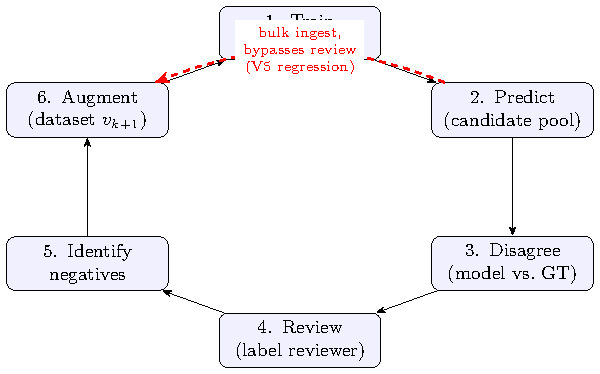
\includegraphics[width=0.62\textwidth]{figures/fig_hitl_loop.pdf}
    \caption{The HITL co-evolution loop. The disciplined path (blue) routes every candidate batch through Disagree$\rightarrow$Review before it is augmented into the next dataset. The V5 regression (Section~\ref{sec:ir_evolution}) took the red shortcut: a large positive batch was ingested directly, bypassing review, so unlabelled drones entered training and were scored as false positives.}
    \label{fig:hitl_loop}
\end{figure}

A model FP is either a real error (hard negative needed) or an annotation error (correct the GT); a model FN is either a real miss (hard positive) or a spurious GT box (remove it). Every disagreement is actionable. The empirical record of this method, the IR detector's six-revision precision/recall trace on a fixed test split including the one revision where the loop was bypassed, is the case study of Section~\ref{sec:ir_evolution}.

\section{Reproducibility Infrastructure}
\label{sec:reproducibility}

Every run writes a \texttt{manifest.json} recording: git commit hash; SHA-256 of loaded weights; CUDA version and device; the full command line; per-frame conf threshold and \texttt{imgsz}; and run timestamps. The cache layer builds a deterministic tag from \texttt{(rgb\_weights\_hash, ir\_weights\_hash, imgsz, stride)}, preventing silent cache reuse across configurations; the unified detection cache (Section~\ref{sec:unified_cache}) extends this to the whole pipeline. Every quantitative claim is registered with its source file, reproduction command, and status. Detector inference is deterministic at fixed weights and conf; the trust classifier (XGBoost) is deterministic at fixed feature input. Only classifier \emph{training} is stochastic, controlled by fixed sequence-stratified group splits.

\section{Model MRI: Feature-Space Analysis}
\label{sec:model_mri}

This thesis follows a \emph{statistics-before-training} discipline: design decisions are settled by measuring what a detector's features encode before any training run. The feature-reuse RGB filter (Section~\ref{sec:distill_verifier}), IR feature separability and grayscale$\leftrightarrow$thermal alignment (Section~\ref{sec:ir_xmodal_verifier}), and trust-classifier feature selection (Section~\ref{sec:feature_selection}) rest on \emph{feature-space} evidence. That evidence is produced by the \emph{Model MRI} tool (\texttt{python -m mri}; modules \texttt{mri/\{extract,classifier,holdout,modality\}.py}).

\subsection{What the Instrument Does}

The tool hooks the detector's FPN layers (\texttt{p3}, stride~8; \texttt{p5}, stride~32) and ROI-pools per-detection activations into a $517$-feature embedding ($512$ pyramid + $5$ detection-metadata scalars), then emits separability statistics, per-layer rankings, spatial activation overlays, and a \texttt{stats.json} keyed to the weight hash and corpus. Each statistic answers a specific sub-question.

\begin{description}
    \item[Linear Discriminant Analysis (LDA).] Projects features onto the Fisher axis maximising between- to within-class variance for drone vs.\ confuser. Threshold accuracy on that axis quantifies linear separability; it is also the visualisation axis of the MRI findings in Section~\ref{sec:mri_findings}.
    \item[ANOVA $F$-statistic.] Per-feature between- to within-class variance ratio; a large $F$ marks a near-binary drone/non-drone switch neuron.
    \item[AUROC.] Probability a random drone outranks a random confuser ($0.5$ chance, $1.0$ perfect); used for the cross-modal transfer test (Section~\ref{sec:ir_xmodal_verifier}) because it requires no operating threshold.
    \item[Leakage ratio.] A second $F$-statistic computed \emph{within} the drone class exposes features that discriminate \emph{which scene} rather than \emph{whether a drone}; the ratio of the two is the feature-selection gate of Section~\ref{sec:feature_selection}.
    \item[Per-modality z-score.] Each feature is standardised to its own modality's $(\mu,\sigma)$; the diagnostic that revealed the grayscale$\leftrightarrow$thermal gap to be a removable affine offset (Section~\ref{sec:ir_xmodal_verifier}).
    \item[CORAL.] Full-covariance alignment (whiten source, re-colour with target covariance), used as the comparison alignment method.
\end{description}

\subsection{From Statistics to a Trained Filter}

The MRI is not only a diagnostic; its output \emph{is} the filter's training pipeline. The same 517-D per-detection embeddings it extracts for analysis become the training matrix for a small MLP, trained automatically with 5-fold cross-validation when the statistics support it (\texttt{mri/classifier.py}); held-out evaluation (\texttt{mri/holdout.py}) gates the result on a corpus excluded from training. The production RGB filter (\texttt{mlp\_v5}) and the cross-modal IR filter (\texttt{mlp\_v5\_ir\_aligned}) are both products of this path: measure first, train only when the measurement says the signal is there, and verify on a held-out gate.

Every run renders a human-readable report. Figure~\ref{fig:mri_report} reproduces the verdict block of the production RGB run verbatim; the full report is in Appendix~\ref{app:mri_report}.

\begin{figure}[htbp]
\begin{quote}\small\ttfamily
\textbf{Model MRI --- Yolo26n\_selcom\_confuser\_ft4\_1280}\\[2pt]
Corpus: 19{,}334 drone / 13{,}597 confuser detections\\[4pt]
\textbf{Verdict: Classifier strongly recommended --- large FP cut at low recall cost.}\\[4pt]
\begin{tabular}{@{}lll@{}}
Signal & Value & Meaning \\
Raw hallucination rate & 54.4\% & bare detector, FP per confuser image \\
LDA separability & 0.952 & linear split of drone vs confuser \\
Max ANOVA $F$ & 42{,}346 & strongest single feature \\
Projected FP cut & 97.4\% & confusers the classifier would reject \\
Recall retention & 98.9\% & true drones the classifier keeps \\
\end{tabular}
\end{quote}
\caption{Excerpt (verbatim) from the Model MRI's auto-generated report for the production RGB detector: the instrument states a verdict, the evidence for it, and the projected operating point of the filter it then trains. Source: \texttt{mri/results/v5\_report\_regen/report.md}.}
\label{fig:mri_report}
\end{figure}

Cross-modal alignment is fit from \emph{drones only} (population-level, no instance pairing) so the confuser transfer test stays independent; headline IR-filter numbers come from a held-out evaluation with CBAM excluded from training. Re-running the MRI on the shipped V5 corpus corrected two figures and one headline claim in an earlier hand-written report: the instrument audits its own paper trail.
% [source: ledger=mri-v5-report-regen; eval=distill_cv_mlp; run=mri/cli.py; cache=mri/results/v5_report_regen/stats.json; config=distill_cv_5fold]

% ======================================================================
% SYSTEM ARCHITECTURE
% ======================================================================
\section{System Architecture and Component Design}
\label{ch:architecture}

\subsection{Overview}

The pipeline processes paired RGB and thermal-IR streams through a four-stage cascade. The production choice for each component is justified by the ablations of Chapter~\ref{ch:hitl}.

\begin{enumerate}
    \item \textbf{RGB detector}: a YOLOv26-class single-stage detector trained on a composite RGB drone corpus that includes bird frames as confuser negatives. Strong on drones; residually hallucinates on small bird-on-sky frames.
    \item \textbf{IR detector}: a YOLOv26-class detector finetuned on iteratively curated thermal imagery (Section~\ref{sec:hitl_method}), with bird, airplane, and helicopter frames as hard negatives. Strong and selective on in-distribution thermal; brittle on OOD thermal. Also operates as a \emph{grayscale-RGB fallback} when no thermal camera is available (Section~\ref{sec:ir_grayscale_mode}).
    \item \textbf{Trust classifier}: an XGBoost model that maps a frame's detection and scene features to a 4-way modality decision (\texttt{reject\_both}, \texttt{trust\_rgb}, \texttt{trust\_ir}, \texttt{trust\_both}).
    \item \textbf{Confuser filter}: in production, the distilled \texttt{mlp\_v5} feature-space filter (Section~\ref{sec:distill_verifier}). Because it reuses the detectors' already-computed ROI features rather than re-processing crops, it is cheap enough to run \emph{per frame} on every detection. It supersedes a 4-class MobileNetV3 patch filter which, being a separate CNN over crop pixels, was expensive enough to require alert-gating (Section~\ref{sec:patch_verifier_arch}).
\end{enumerate}

A temporal smoother sits on top of the cascade: it raises an alert only when the per-frame decision has persisted across a configurable sliding window. In the predecessor design the smoother also gated the (expensive) patch filter. The per-frame \texttt{mlp\_v5} filter removes that coupling, so the alert-gate analysis of Section~\ref{sec:alert_gate} now describes the superseded patch path.

\begin{figure}[htbp]
    \centering
    
\includegraphics[width=\textwidth]{figures/fig_pipeline.pdf}
    \caption{Multi-stage drone detection pipeline. The production confuser filter is the distilled \texttt{mlp\_v5}, which runs \textbf{per frame} because it reuses the detectors' already-computed ROI features rather than re-processing crops (Section~\ref{sec:distill_verifier}). It supersedes the MobileNetV3 patch filter (greyed), which was expensive enough that it had to be \emph{alert-gated}: consulted only when the temporal smoother was about to fire (Section~\ref{sec:alert_gate}).}
    \label{fig:pipeline}
\end{figure}

The downstream stages contribute the majority of confuser suppression without retraining the detectors. Three architectural choices make this possible: fail-open detection (Section~\ref{sec:design_rationale}), trust-aware fusion (Section~\ref{sec:trust_fusion}), and a downstream per-frame confuser filter.

\paragraph{Two-filter fusion (trust-first).} With both RGB (\texttt{mlp\_v5}) and IR (\texttt{mlp\_v5\_ir\_aligned}) filters running per-frame, fusion is \emph{trust-first}: the trust classifier (Section~\ref{sec:trust_fusion}) routes, then the trusted modality's confuser filter screens the surviving detections. \texttt{reject\_both} drops the frame; \texttt{trust\_rgb} keeps it only if the RGB filter passes; \texttt{trust\_ir} keeps it only if the IR filter passes; \texttt{trust\_both} is resolved per-modality (recall-first: the detection survives if either trusted filter passes). The IR filter is one network with two per-modality input scalers (a thermal scaler and a grayscale scaler), so a single trained filter serves both the thermal-deploy and grayscale-fallback paths (Section~\ref{sec:ir_xmodal_verifier}). The composition order (classifier$\to$filter vs filter$\to$classifier) is itself ablated in Section~\ref{sec:pipeline_ablation}.
% [source: ledger=dual-filter-fusion-rule]

\subsection{Design Rationale: Fail-Open}
\label{sec:design_rationale}

The cascade's central design principle is asymmetric recoverability: a confuser false positive raised by the detector can be vetoed downstream, but a drone the detector missed cannot be recovered by any later stage. The cascade therefore ``fails open'' at the detector, deferring suppression rather than suppressing early at the cost of unrecoverable misses. Both detectors are trained with confuser negatives (Section~\ref{sec:rgb_three_variants}, Section~\ref{sec:ir_detector}), but training-time mining does not eliminate all categories: bird hallucination at the RGB detector is irreducible at small drone sizes, as the three-stance comparison shows: the stance that suppresses birds (\texttt{retrained\_v2}, bird fire $94.4\% \to 3.4\%$) collapses Svanstr\"om drone recall $0.961 \to 0.306$ (Table~\ref{tab:rgb_comparison}, Section~\ref{sec:rgb_results}). The cascade is built around that residual: the downstream stages catch what training cannot, at a cost and benefit quantified stage-by-stage in Section~\ref{sec:pipeline_ablation}.
% [source: ledger=retrainedv2-recall-collapse; eval=rgb_svan_retrainedv2; cache=eval/results/_failure_diagnosis/svanstrom_1280_by_category.csv; config=svan_iop_1280]

\subsection{Trust-Aware Fusion}
\label{sec:trust_fusion}

The fusion stage is a learned per-frame decision rather than a fixed vote. The classifier outputs one of four labels:

\begin{itemize}
    \item \textbf{\texttt{reject\_both}}, neither modality's detection is trustworthy (likely a confuser).
    \item \textbf{\texttt{trust\_rgb}}, only RGB is reliable for this frame.
    \item \textbf{\texttt{trust\_ir}}, only IR is reliable for this frame.
    \item \textbf{\texttt{trust\_both}}, both modalities agree and are trustworthy.
\end{itemize}

The 4-way formulation captures \emph{when} each modality is reliable. The asymmetry the classifier exploits is that \emph{the two detectors hallucinate on different scenes}: visual confusers fool the RGB detector more reliably; thermally degraded conditions fool the IR detector more reliably. A per-frame classifier can pick the modality whose failure profile is least active; a fixed-weight rule cannot. The per-surface evidence, including the modality reversal between Svanstr\"om (IR stronger) and Anti-UAV (RGB stronger) that makes routing pay, is in Section~\ref{sec:pipeline_ablation}.

The production router is the eight-feature leakage-aware \texttt{robust8} (Section~\ref{sec:feature_selection}); the hand-engineered 32-feature \texttt{sa32} serves as the strongest classical comparison throughout the evaluation.

\subsection{Alert-Gate Cascade (superseded patch path)}
\label{sec:alert_gate}

This section describes the MobileNetV3 \emph{patch} filter's position in the predecessor design, retained because part of the historical evidence was measured under it. Alert-gating was forced by the patch filter's cost (a second CNN over crop pixels): the filter was consulted only when the temporal smoother was about to emit an alert. Two alternative cascades were considered and rejected at the time (\texttt{filter\_then\_classifier} and \texttt{classifier\_then\_filter} as \emph{per-frame patch} stages), because the patch CNN's per-frame cost and its veto of marginal drone TPs cost $\approx$1~pp Svanstr\"om F1. The per-frame \texttt{mlp\_v5} filter removes the cost argument entirely, and the composition-order question is re-answered with it in Section~\ref{sec:pipeline_ablation}. The production GUI path is implemented in \texttt{ir\_gui/pyside\_engine.py} (\texttt{should\_suppress\_alert}).

\subsection{Temporal Smoother}
\label{sec:temporal}

The temporal smoother is an $N$-of-$M$ sliding-window aggregator with configurable cooldown. An alert fires only when the trust classifier's per-frame decision has been positive on at least $N$ of the last $M$ frames, absorbing isolated firings characteristic of birds and aircraft transiting the field of view. Its measured contribution, at the segment grain on the real-video clips, is in Section~\ref{sec:temporal_results}.

The same temporal state drives a \emph{ROI fallback} in the PySide engine (\texttt{\_run\_with\_roi}). When the full-frame YOLO returns nothing and a recent track is still alive, YOLO is re-run on an expanded crop around the previous box at reduced confidence. This is a GUI-only feature, and the frame-mode evaluation harness does not use it; it accounts for part of the GUI-versus-eval performance gap on small distant drones. The GUI maintains tracks and renders a path image, but does not yet classify on track-level features (flight dynamics); track-level classification is a future-work direction.

\begin{figure}[htbp]
    \centering
    \fbox{\parbox{0.9\textwidth}{\centering\vspace{2cm}
        \textbf{[PLACEHOLDER: PySide6 deployment GUI]} Annotated screenshot of the deployed GUI: dual-modality view (RGB + IR side by side), per-frame trust-label readout, sliding temporal window indicator, alert banner, ROI fallback crop inset, drone-path overlay across recent frames, threshold sliders for RGB / IR / filter.
    \vspace{2cm}}}
    \caption{PySide6 operator GUI. The temporal smoother's state, the trust classifier's per-frame decision, and the ROI fallback crop are all surfaced for the human operator.}
    \label{fig:pyside_gui}
\end{figure}

\subsection{Resolution Dependency}
\label{sec:resolution_arch}

Resolution is the single largest hyperparameter affecting small-drone recall. Svanstr\"om's native resolution is $640\times 512$; at \texttt{imgsz=1280} the baseline RGB detector reaches $R=0.961$ on Svanstr\"om drones, whereas at \texttt{imgsz=640} small drones fall below the resolvable floor (\texttt{retrained\_v2} collapses to $R=0.072$ at that size). Anti-UAV imagery ($1920\times 1080$) saturates at \texttt{imgsz=640} because drones already span enough pixels. All Svanstr\"om RGB evaluation uses \texttt{imgsz=1280} (Section~\ref{sec:canonical_configs}). SelCom CCTV is a third regime: clutter is the binding constraint, and the imgsz sweep identifies $\mathtt{imgsz}=960$ as the F1-optimal setting for that camera's deployment operating point.
% [source: ledger=selcom-imgsz-win; eval=rgb_svan_baseline; run=eval/diagnose_failures.py; cache=eval/results/_failure_diagnosis/svanstrom_1280_by_category.csv; config=svan_iop_1280]

\begin{figure}[htbp]
    \centering
    
\includegraphics[width=0.85\textwidth]{fig6_6_resolution}
    \caption{Inference-resolution dependency of Svanstr\"om drone recall. At \texttt{imgsz=1280} the baseline detector reaches $R=0.961$; the \texttt{imgsz=640} floor is illustrated with \texttt{retrained\_v2} ($R=0.072$), the only variant measured at that size; the baseline's own \texttt{imgsz=640} run is pending, so the two endpoints are different variants and the curve is indicative, not a single-model sweep.}
    % [source: ledger=retrainedv2-recall-collapse; eval=rgb_svan_baseline; run=eval/diagnose_failures.py; cache=eval/results/_failure_diagnosis/svanstrom_1280_by_category.csv; config=svan_iop_1280]
    \label{fig:resolution}
\end{figure}

\subsection{RGB Drone Detector}
\label{sec:rgb_detector}

The RGB detector is a YOLOv26n (nano) single-class detector trained on the composite corpus of Section~\ref{sec:ds_rgb_corpus}, which includes a drone-vs-bird subset as deliberate confuser negatives. Svanstr\"om imagery is held out from training.

\subsubsection{Three Training Stances}
\label{sec:rgb_three_variants}

Three RGB-detector variants explore how much additional confuser-specific data to add on top of the baseline corpus; they occupy three operating points on the recall--hallucination axis, and their full comparison is Table~\ref{tab:rgb_comparison} (Section~\ref{sec:rgb_results}).

\begin{enumerate}
    \item \textbf{Baseline} (\texttt{Yolo26n\_trained}). Trained on the composite drone corpus. On Svanstr\"om@1280 it reaches $P=0.940, R=0.961$ on drones, with a 94.4\% bird-frame fire rate.
    \item \textbf{\texttt{hardneg\_v3more}}. Same backbone, retrained with the Svanstr\"om bird/airplane/helicopter confuser splits supplied as additional negatives. Helicopter fire drops $66.2\% \to 41.9\%$ and airplane $74.6\% \to 64.7\%$, while bird fire is essentially unchanged ($94.2\%$): hard-negative mining is class-specific.
    \item \textbf{\texttt{retrained\_v2}}. Aggressive retraining with heavy confuser augmentation. Bird fire collapses to 3.4\%, and Svanstr\"om drone recall collapses with it, to $R=0.306$. The lesson that motivated the cascade: at small drone scales, bird suppression and drone recall cannot both be had at the detector.
\end{enumerate}
% [source: ledger=retrainedv2-recall-collapse; eval=rgb_svan_baseline,rgb_svan_hardneg,rgb_svan_retrainedv2; cache=eval/results/_failure_diagnosis/svanstrom_1280_by_category.csv; config=svan_iop_1280]

The production RGB detector, \texttt{ft4} (\texttt{Yolo26n\_selcom\_confuser\_ft4\_1280}), is a fourth stance built on the lessons of the first three: the SelCom fine-tune line (Section~\ref{sec:selcom_finetune}) plus a \emph{regression-gated} confuser injection (300 hard negatives at \texttt{freeze}$=$15; Section~\ref{sec:training_recipes}) that cut confuser hallucination 16~pp without recall loss.

\subsubsection{SelCom CCTV Fine-Tune}
\label{sec:selcom_finetune}

A separate fine-tune line targets the deployment partner's CCTV stream (Section~\ref{sec:ds_selcom}). The fine-tune is on top of the \emph{baseline} weights (not \texttt{retrained\_v2}), keeping the cascade compatible with the deployed classifier without a recalibration swap. Two mixed-training fine-tunes (80\% general RGB + 20\% selcom; pure-selcom val split, seed 0) were trained at 640 and 1280; the 1280 variant doubles SelCom recall \emph{and} raises precision over its 640 sibling (Table~\ref{tab:selcom}, Section~\ref{sec:rgb_results}), the clearest single demonstration that resolution, not architecture, is the binding constraint on small-drone CCTV. A preprocessing sweep established that no OpenCV variant (denoise, CLAHE, sharpen, contrast) improves detection independently of fine-tuning and \texttt{imgsz}; the imgsz sweep identifies 960 as the F1-optimal deployment point for this camera. The regression on the standard RGB dataset is within $-0.008$ F1 of baseline.
% [source: ledger=selcom-imgsz-win; eval=selcom_ft2_1280; run=RGB model/finetune_selcom.py; cache=runs/rgb_finetune_eval/Yolo26n_selcom_mixed_ft2_1280/comparison.json; config=selcom_iop_1280]

\subsection{IR Drone Detector}
\label{sec:ir_detector}

The IR detector uses the same YOLOv26n architecture finetuned on iteratively curated thermal data via the HITL engine (Section~\ref{sec:hitl_method}). Bird, airplane, and helicopter thermal frames are added as hard negatives across revisions. The production weights (\texttt{v3b}) are a 2-epoch corrective fine-tune on the \texttt{Final} checkpoint addressing specific deployment-time failure modes. The full evolution across six numbered revisions (including the V5 regression and its recovery) is the case study of Section~\ref{sec:ir_evolution}; on the paired benchmarks the IR detector is the stronger single-modality detector on Svanstr\"om and the weaker one on Anti-UAV (Section~\ref{sec:pipeline_ablation}), which is precisely the asymmetry the trust classifier exploits.

\subsubsection{Grayscale-RGB Operating Mode}
\label{sec:ir_grayscale_mode}

The deployed PySide GUI exposes a \emph{grayscale-RGB} operating mode (\texttt{\_infer\_grayscale}). When no thermal camera is available, the GUI converts the RGB stream to grayscale via \texttt{cvtColor(BGR2GRAY)}, replicates to three channels, and feeds the result to the IR detector at \texttt{imgsz=640}. This was built as a conservative hardware fallback; its measured behaviour (competitive with the dedicated RGB detector on bird-cluttered scenes, a few points behind it overall) turned out to be one of the thesis's findings (Section~\ref{sec:grayscale}).

\subsubsection{Cross-Modal Feature Alignment: a Thermal Filter from Grayscale Confusers}
\label{sec:ir_xmodal_verifier}

The same grayscale mode dissolves the data-scarcity blocker that had previously kept a per-frame IR confuser filter out of the production stack. Labelled thermal confusers are rare; grayscale-RGB confusers are abundant. Two Model MRI measurements make the harvest usable (evidence figures in Section~\ref{sec:mri_findings}):

\emph{First, the confuser-rejection signal already lives inside the IR detector.} An MRI of the \texttt{v3b} fused \texttt{p3}+\texttt{p5} ROI features over $14{,}697$ drone and $1{,}386$ confuser detections shows near-linear separability (single linear discriminant: $0.981$ train accuracy; strongest neuron ANOVA $F=5{,}370$). The IR feature space is the thermal twin of the RGB filter's, readable by the same kind of lightweight MLP with no detector retraining.
% [source: ledger=ir-features-separable; run=mri/cli.py; cache=mri/results/ir_v3b_report; config=ir_v3b]

\emph{Second, the grayscale$\rightarrow$thermal feature gap is a removable affine offset.} The detector represents a given class almost identically in real thermal and in grayscale-RGB (top-discriminative-neuron overlap Jaccard $0.71$--$0.88$; mean-activation correlation $0.93$--$0.99$; drone-centroid cosine distance $0.012$); the only systematic difference is a per-feature mean/scale offset. Removing it with a per-modality z-score lifts grayscale$\rightarrow$thermal confuser-transfer AUROC from $0.500$ (chance) to $0.919$ against a within-thermal ceiling of $0.974$; full-covariance CORAL reaches only $0.707$, confirming the gap is diagonal.
% [source: ledger=gray-thermal-alignable; run=mri/modality_align.py; cache=mri/results/ir_v3b_report; config=ir_v3b]

The production checkpoint \texttt{mlp\_v5\_ir\_aligned} therefore combines thermal drone detections (for recall safety; a $\sim$30k drone-diversity re-mine made the filter recall-safe on held-out thermal) with grayscale-harvested confusers, per-modality z-aligned into a single $517$-D filter. It is \emph{one network with two per-modality input scalers}: a thermal scaler and a grayscale scaler share the same weights and differ only in the $(\mu,\sigma)$ standardisation folded into the input, so a single trained filter serves both the thermal-deploy and grayscale-fallback paths. CBAM, a novel thermal aerial-confuser set, is held out of its training; the held-out results are in Section~\ref{sec:verifier_results}.
% [source: ledger=ir-grayscale-harvest-solves-thermal-filter,ir-recall-fixed-by-drone-diversity]

\subsection{Trust Classifier}
\label{sec:trust_classifier}

\subsubsection{Feature Set}

The trust classifier consumes per-frame features from the two detectors' raw outputs and the source frames. The shipped classifier is the eight-feature \texttt{robust8} (Section~\ref{sec:feature_selection}); the hand-engineered comparison set is \texttt{sa32} (32 features) and two 40-feature variants. The feature families:

\begin{itemize}
    \item \textbf{Detector signals}: per-modality binary detection flags, top-$k$ confidence scores, detection counts.
    \item \textbf{Scene features}: image intensity statistics, edge density, frequency-domain summaries; intended to detect ``confuser-rich'' scenes vs ``clean sky'' scenes; as Section~\ref{sec:feature_selection} shows, also the family that leaks scene identity.
    \item \textbf{Target features}: bounding-box geometry (aspect ratio, normalised area, position), confidence distribution per modality.
    \item \textbf{Agreement features}: cross-modal IoU, centre distance, confidence ratio.
    \item \textbf{Failure-model scores} (only in \texttt{control\_v3more\_40feat}): scalar outputs from a small per-modality failure-prediction network, dropped in later variants because they over-fitted to training-set artefacts.
\end{itemize}

The label space is the 4-way trust decision of Section~\ref{sec:trust_fusion}. The model is an XGBoost~\cite{chen2016xgboost} gradient-boosted classifier. Training uses sequence-stratified group shuffling so that frames from a given sequence are not split across train and test. The Svanstr\"om overlap this leaves at the cascade level is flagged in Section~\ref{sec:svanstrom_audit}.

\subsubsection{Hand-Engineered Variants (the comparison set)}
\label{sec:classifier_variants}

Three hand-engineered variants preceded the statistical selection: \texttt{sa32} (\texttt{scene\_aware\_v3more\_32feat}; the strongest, and the working production pick through the real-video comparison), \texttt{fusion\_no\_fn\_v1.1} (the most conservative on OOD confusers; rejects most drone TPs on operational video; retained as an open-world fallback where missed drones are operationally tolerable), and \texttt{control\_v3more\_40feat} (deprecated; no surface favours it). Their quantitative comparison, and the surface reversal between Svanstr\"om and real video that it revealed, is in Section~\ref{sec:classifier_results}.

The early \texttt{retrained\_v2\_32feat} classifier is superseded because the production RGB detector is no longer \texttt{retrained\_v2}; a training-time/production confidence-distribution mismatch accounts for most of its gap. A trust classifier is not portable across RGB detector swaps without re-checking calibration.

\paragraph{Scene-fingerprint over-fitting.}
Under sequence-stratified splitting, per-clip image statistics act as \emph{scene fingerprints}: the classifier learns which clip a frame came from rather than whether a drone is present, inflating in-distribution scores while degrading transfer. Dropping these features (the \texttt{lean13}$\to$\texttt{lean10} pruning) recovers $18$--$26$~pp drone $F1$ on held-out clips. Section~\ref{sec:feature_selection} turns this hindsight observation into a statistic computed before training.
% [source: ledger=scene-fingerprint-overfit; eval=own_lean10_yt,own_lean13_yt; config=clf_own_holdout]

\subsubsection{Statistical Feature Selection: \texttt{robust6} and \texttt{robust8}}
\label{sec:feature_selection}

The variants above were assembled by hand; this subsection replaces that procedure with a statistical one. Two practical pressures sharpen the motivating question: \texttt{sa32} was trained on detections from a superseded detector (its inputs no longer match the production \texttt{ft4}/\texttt{v3b}), and several of its features require an expensive per-frame OpenCV pass.

\paragraph{Method.}
From a cached $56$-feature matrix of $65{,}192$ frames we ran four analyses. LDA asks whether the signal is present: a single Fisher axis separates trust-positive from reject at $98.2\%$ training accuracy (Figure~\ref{fig:fusion_lda}), so the problem is \emph{selecting} features, not a signal shortage. PCA asks whether the structure is trivial: classes overlap in the top components, meaning scene-to-scene variance dominates over the drone signal. A per-feature ANOVA $F$-test and single-feature AUROC then rank each feature individually (Figure~\ref{fig:fusion_auroc}).
% [source: ledger=fusion-feature-leakage; run=classifier/fusion_feature_stats.py; cache=classifier/fusion_models/optimal_v1/feature_stats_ranked.csv; config=clf_own_holdout]

\paragraph{A leakage statistic.}
A scene-fingerprint feature can score as discriminative in a single pool simply because it correlates with which scene a sample came from; ANOVA and AUROC would recommend keeping it. To expose this we compute a second $F$-statistic \emph{within the drone class only} and form the ratio
\begin{equation}
\mathit{leakage\_ratio} = \frac{F_\text{domain-in-class}}{F_\text{class}},
\label{eq:leakage}
\end{equation}
which is low for a robust signal feature and high for a scene fingerprint. Equation~\ref{eq:leakage} converts the earlier hand-tuned deprecations into a number computed before any training run.
% [source: ledger=fusion-feature-leakage; run=classifier/fusion_feature_stats.py; cache=classifier/fusion_models/optimal_v1/feature_stats_ranked.csv; config=clf_own_holdout]

\begin{figure}[htbp]
    \centering
    \begin{subfigure}{0.32\textwidth}
\includegraphics[width=\textwidth]{fig8_fusion_lda}\caption{}\label{fig:fusion_lda}\end{subfigure}
    \hfill
    \begin{subfigure}{0.32\textwidth}
\includegraphics[width=\textwidth]{fig8_fusion_auroc}\caption{}\label{fig:fusion_auroc}\end{subfigure}
    \hfill
    \begin{subfigure}{0.32\textwidth}
\includegraphics[width=\textwidth]{fig8_fusion_leakage}\caption{}\label{fig:fusion_leakage}\end{subfigure}
    \caption{Statistical anatomy of the $56$-feature fusion space. (a) Linear discriminant: the trust signal is linearly separable ($98.2\%$ train accuracy). (b) Per-feature single-feature AUROC. (c) Leakage map (Eq.~\ref{eq:leakage}): the lower-right region is robust signal (high AUROC, near-zero leakage); the upper-left is scene fingerprint (chance-level AUROC, leakage in the hundreds). Source: \texttt{classifier/fusion\_feature\_stats.py}.}
    % [source: ledger=fusion-feature-leakage; run=classifier/fusion_feature_stats.py; cache=classifier/fusion_models/optimal_v1/feature_stats_ranked.csv; config=clf_own_holdout]
    \label{fig:fusion_stats}
\end{figure}

\paragraph{What the statistic finds.}
The leakage map separates two groups cleanly (Table~\ref{tab:leakage}). Scene-statistic features score at chance on the class label yet have leakage ratios in the hundreds: they discriminate \emph{which scene}, not whether a drone is present, and are also the expensive per-frame features. The robust core (detection confidences, box geometry, and cross-modal ratios) scores AUROC above $0.9$ with leakage below $0.006$. A within-source check catches what the leakage ratio misses: \texttt{rgb\_blurriness} scores AUROC $0.872$ in the pooled set but collapses to $0.516$ within each source (a cross-clip mean-shift artefact), so the gate drops it alongside the scene fingerprints. Two caveats. Per-modality detection-presence flags top the AUROC chart but are excluded by reasoning, since the trust label is \emph{derived from} those detections. And the corpus is IR-dominant, so IR features rank above their RGB counterparts on RGB-fallback surfaces.
% [source: ledger=fusion-feature-leakage,blurriness-is-corpus-artifact; run=classifier/fusion_feature_stats.py,classifier/vet_blurriness_stats.py; cache=classifier/fusion_models/optimal_v1/feature_stats_ranked.csv; config=clf_own_holdout]

\begin{table}[htbp]
    \centering
    \caption{Leakage analysis splits the feature space. \emph{Top}: scene fingerprints, chance-level class AUROC but very high leakage; drop. \emph{Bottom}: the robust core, high AUROC, near-zero leakage; keep. Source: \texttt{feature\_stats\_ranked.csv}.}
    \label{tab:leakage}
    \begin{tabular}{llcc}
        \toprule
        feature & family & AUROC-alone & leakage ratio \\
        \midrule
        \multicolumn{4}{l}{\emph{Scene fingerprints (drop)}} \\
        \texttt{rgb\_img\_std}       & scene       & 0.502 & 349.6 \\
        \texttt{rgb\_img\_entropy}   & scene       & 0.510 & 307.4 \\
        \texttt{ir\_blurriness}      & scene       & 0.795 & 11.7 \\
        \texttt{rgb\_edge\_density}  & scene       & 0.525 & 1.75 \\
        \midrule
        \multicolumn{4}{l}{\emph{Robust core (keep)}} \\
        \texttt{conf\_sum}             & confidence  & 0.983 & 0.002 \\
        \texttt{ir\_max\_conf}         & confidence  & 0.965 & 0.002 \\
        \texttt{ir\_best\_aspect\_ratio} & geometry  & 0.952 & 0.002 \\
        \texttt{ir\_best\_log\_bbox\_area} & geometry & 0.946 & 0.005 \\
        \texttt{xmodal\_conf\_ratio}   & cross-modal & 0.905 & 0.002 \\
        \bottomrule
    \end{tabular}
\end{table}

\paragraph{\texttt{robust6}.}
Applying the keep rule yields \texttt{robust6} $=$ \{\texttt{rgb\_max\_conf}, \texttt{ir\_max\_conf}, \texttt{rgb\_best\_log\_bbox\_area}, \texttt{ir\_best\_log\_bbox\_area}, \texttt{rgb\_best\_aspect\_ratio}, \texttt{ir\_best\_aspect\_ratio}\}: all free detector outputs and box geometry, all near-zero leakage. Training data is re-mined from the current \texttt{ft4}/\texttt{v3b} detectors, fixing the drift in \texttt{sa32}'s inputs. Two ablation levels confirm the design: in-domain $F1$ is flat as the feature count grows from $6$ to $32$ (count is not the lever), but on OOD drone video the set \emph{with} fingerprint features collapses to $F1=0.262$, climbing to $0.578$ for \texttt{robust6}; dropping fingerprints roughly doubles OOD generalisation. Dropping IR geometry also loses confuser rejection, so box-geometry features are load-bearing.
% [source: ledger=ft4-lean-trust-classifier; run=classifier/train_lean_ft4.py; cache=docs/analysis/2026-05-31_ft4_lean_trust_classifier.md; config=clf_own_holdout]

\paragraph{Closing the grayscale hole: \texttt{robust8}.}
\texttt{robust6} inherits one honest weakness from its lean feature set: in the grayscale-RGB fallback regime its IR-side features go uninformative, drone-only-in-RGB frames are routed to \texttt{reject}, and grayscale drone recall collapses. The fix is statistical, not architectural: on the affected slice, \texttt{rgb\_mean\_conf} separates drone from confuser at AUROC $0.934$, a learned object signal the six-feature set omitted. Adding it with an \texttt{is\_grayscale} regime flag gives the eight-feature \texttt{robust8}; a per-class threshold $\tau$ on $P(\texttt{trust\_rgb})$ ($\tau=0.20$ shipped) converts the now-present signal into recall. Validated end-to-end, \texttt{robust8} lifts Svanstr\"om-grayscale drone recall $0.577 \to 0.681$ at unchanged precision and ties thermal $F1$; the structural cost (a $7$--$10\times$ real-video-confuser fire increase on that slice) is reported with it in Section~\ref{sec:classifier_results}.
% [source: ledger=robust8-grayscale-router; eval=svan_gray_robust8_t20_clffilter; run=eval/compare_routing_pipeline.py; cache=eval/results/_routing_pipeline_cmp/comparison.md]

\paragraph{Further free levers.}
Forward selection surfaces cross-modal difference features (\texttt{pos\_euclidean\_diff}, \texttt{area\_diff}) that beat the expensive scene statistics on grayscale routing (macro-$F1$ $0.36 \to 0.61$). A stronger lever is the filter's own output: \texttt{mlp\_v5} drone probability separates trust-positive from reject at AUROC $0.949$ vs $0.842$ for raw confidence. It is withheld from \texttt{robust8} because coupling the filter into the classifier introduces stage dependency; it is recorded as the next free lever.
% [source: ledger=forward-selection-free-xmodal-diffs-win,filter-score-as-classifier-feature; run=classifier/forward_select_routing.py,classifier/verifier_as_feature_stats.py; cache=docs/analysis/2026-06-02_forward_selection_study.md]

\subsection{Patch Filter (Superseded Predecessor)}
\label{sec:patch_verifier_arch}

This section documents the \emph{predecessor} confuser filter, retained because part of the historical evidence was measured against it; the production filter is \texttt{mlp\_v5} (Section~\ref{sec:distill_verifier}).

The patch filter is a 4-class image classifier (\texttt{airplane} / \texttt{helicopter} / \texttt{bird} / \texttt{other}) on a MobileNetV3-Small backbone~\cite{howard2019mobilenetv3}, chosen because it fits within a YOLO-forward-pass budget on the GTX 1050 Ti development hardware. It was trained on \textbf{45{,}917 RGB+IR patches}: drone crops taken from the detector training corpora's ground-truth boxes, and bird/airplane/helicopter crops hard-negative-mined from detector false positives over the confuser corpus (Section~\ref{sec:ds_confusers}) and OOD YouTube video (\texttt{classifier/extract\_patches\_v2.py}); no CCTV crops are included. Per-modality twins are trained (\texttt{confuser\_filter4\_\{rgb,ir\}\_v2}). On its own validation split it reaches accuracy $0.975$, with per-class precision/recall of $0.907/0.971$ (airplane), $0.988/0.938$ (helicopter), and $0.893/0.712$ (bird); birds were already the weakest class at training time, foreshadowing the deployment gap.
% [source: models.csv patch_v2 (train_dataset=45,917 patches); cache=classifier/runs/patches/confuser_filter4_rgb_metrics.json]

At inference the filter consumes the YOLO crop and emits a softmax over the four classes; the veto uses $p_\text{confuser} = \max(p_\text{airplane}, p_\text{helicopter}, p_\text{bird})$ thresholded at \texttt{patch\_thr}. The \texttt{other} class is an explicit OOD outlet: crops that look neither like a trained confuser nor like a drone route to \texttt{other} instead of being forced into a confuser class. Four numbered versions exist; v2 is the audited production version (v3 over-vetoes and is never shipped; v4 ties v2). Its threshold sweep, per-category catch rates, and the cost analysis that motivated its replacement are in Section~\ref{sec:verifier_results}.
% [source: ledger=patch-version-ranking,patch-catch-below-bar]

\subsection{Feature-Reuse Filter (\texttt{mlp\_v5})}
\label{sec:distill_verifier}

The patch filter re-processes each detection crop with a network entirely separate from the detector; on unseen surfaces it abstains to \texttt{other} (on SelCom CCTV it is bit-for-bit identical to the bare detector, having never seen CCTV-scale crops). This motivates a structurally different filter.
% [source: ledger=patch-v2-neutral-selcom; eval=v5_selcom_patch; config=selcom_iop_1280]

The \emph{feature-reuse filter} replaces pixel re-processing with feature reuse: a small MLP consumes the RGB detector's own fused \texttt{p3}+\texttt{p5} ROI activations, already computed for each candidate box, ROI-pooled to a 512-D embedding plus 5 metadata scalars ($517$ features total). The Model MRI characterised these features on the $32{,}931$-detection corpus the shipped \texttt{mlp\_v5} was trained on ($19{,}334$ drone / $13{,}597$ confuser detections mined across the RGB surfaces): a single linear discriminant separates drone from confuser at ${\approx}95\%$ train accuracy, while unsupervised PCA shows near-zero cluster separation (silhouette $0.067$): the signal is real but lives in a supervised subspace, so it needs a trained classifier rather than a distance threshold. The MRI findings, including the activation ``brain scans'' of what the filter reads, are in Section~\ref{sec:mri_findings}; the filter's measured effect on every surface is in Section~\ref{sec:verifier_results}.
% [source: ledger=v5-lda-separability; eval=distill_cv_mlp; run=mri/cli.py; cache=mri/results/v5_report_regen/stats.json; config=distill_cv_5fold]

Feature reuse makes the filter $46$--$72\times$ faster per detection than the patch CNN ($1.3$--$2.1$~ms vs $59$--$112$~ms; $1$--$4\%$ pipeline overhead), which is what makes \emph{per-frame} verification affordable and removes the alert-gate coupling of the predecessor design. On the shipped corpus the MLP reaches 5-fold CV $F1$ of $0.9857\pm0.0004$, rejecting $97\%$ of confuser detections while retaining $98.9\%$ of true drones. Its IR counterpart, \texttt{mlp\_v5\_ir\_aligned}, is the cross-modal product of Section~\ref{sec:ir_xmodal_verifier}: one network, two per-modality input scalers, serving thermal and grayscale-fed channels alike.
% [source: ledger=v5-ship-per-frame,embedding-distillation-cv; run=eval/bench_speed.py]
